\documentclass{article}

\usepackage{amsmath}
\usepackage{amsfonts}
\usepackage{graphicx}
\usepackage{cite}
\usepackage[square,numbers]{natbib}

\begin{document}

\section{Introduction}
Empirical Risk Minimisation (ERM) is a principle of statistical theory that is used in supervised learning. Simply put, it states that for a function to make the most accurate predictions possible on an unknown true distribution, prediction errors made on the data belonging to the distribution must be minimised. To give a proper explanation of the principle some prior concepts need to be explained. The next section will discuss loss functions. 

\section{Loss Functions}
A simple supervised learning scenario comprises of the following. Typically there would be one or more inputs or features denoted as $x$ and the target output or labels denoted as $y$.
Using the combination of features and output $(x,y)$, a prediction function $f(x)$ is built where, given a new input $x'$ gives the best estimate for the value of $y'$, assuming that the data follows an underlying distribution that is not known. Once a set of predictions is generated, a way of measuring how good these predictions are is required. For a single data point this is simply the distance between $y$ and $y'$. Repeating this process for multiple points will give us a loss function \citep{Wehenkel2018}:
\begin{equation}
    L(f(x),y)
\end{equation}
The loss function gives us the cost our prediction function (f(x)) which gives a clear indication of how efficient the function is at predicting the expected output. Common loss functions are squared-error loss  and mean square error. This calculation of "cost" of the function can give us an indication of the risk of the prediction function. Therefore, the goal of finding the most optimal prediction function turns out to be the goal of finding the function which minimises the true risk.

\section{True Risk}

True Risk is the prediction error on the entire population of data. In almost all cases, it is impossible to collect the entire data as it almost impossible. For example, in the case of predicting the gender of a person based on their height and weight, every single person across the globe would need to have their height and weight collected all into one set of data. Since entire population is not available there needs to be a way of minimising the true risk, without the true distribution being known. 

\section{Empirical Risk Minimisation}
This is where Empirical Risk Minimisation comes in. When constructing the supervised learning model, the predictive function chosen is the one with the  least discrepancy between predicted values and actual values. In other words, the one with the least risk. This risk is Empirical Risk and the process of finding the function that minimises the risk is Empirical Risk Minimisation. Note the risk is empirical risk and not the true risk as the data is only subset of the entire population. In an ideal scenario the end goal would be to minimise the true risk as much as possible. Due to the fact that the data for calculating the true risk is unavailable this cannot be achieved, however it is said that the empirical risk is almost identical to true risk. Therefore by minimising the empirical risk the true risk should be minimised also.

\section{Equation of Empirical Risk Minimisation}

The following is the equation for the Empirical Risk Minimisation as proposed by \citet{Vapnik}\citep{principles}:

\begin{equation}
    R_{emp}(f) = \frac{1}{m} \sum_{i=1}^{m} L(f(x_{i})   ,y_{i}).
\end{equation}
Here $R_{emp}$ denotes the empirical risk or empirical error for a particular prediction function $f(x)$. The number of input and output pairs is denoted as m. As can be seen in the equation above, empirical risk equates to the sum average of the of the loss function on each pair of $x$ and $y$ points generated. The induction principle behind empirical risk minimisation makes the assumption that the prediction function $f(x)$, which minimises the risk $R_{emp}$, will result in a risk $R_{emp}*$ which is close to its minimum. 

\section{Uniform Convergence}
The convergence of the empirical risk to the true risk can only be achieved under specific conditions and bounds \citep{Clemencon2017}. These bounds are independent of the prediction function and are based on the VC-dimension of the dataset. This dimension basically measures the complexity of the prediction function. The VC-Dimension set also measures ability of the function to perform correct predictions on unseen data, using the least training data possible. A low VC Dimension indicates a high bias in the function, which will lead the function to perform poorly (especially on training data) as it will cause underfitting. On the other hand, a high VC-Dimension which indicates that the function has a high complexity. The complexity could be high to the point that the function would memorise the data rather than idenitfy the underlying pattern which causes overfitting. Based on this, prediction function with high complexity should be avoided. When comparing two fcuntions which have roughly the same empirical error, the least complex one should be chosen in order to avoid the scenario of overfitting.

\section{Problem of Empirical Risk Minimisation}
The most common problem of ERM as mentioned above is overfitting. As the goal is to reduce the empirical error as much as possible, the result could be a prediction function that fits the training data perfectly. However when given unseen data this will perform poorly causing overfitting \citep{UMachineLearning}. 

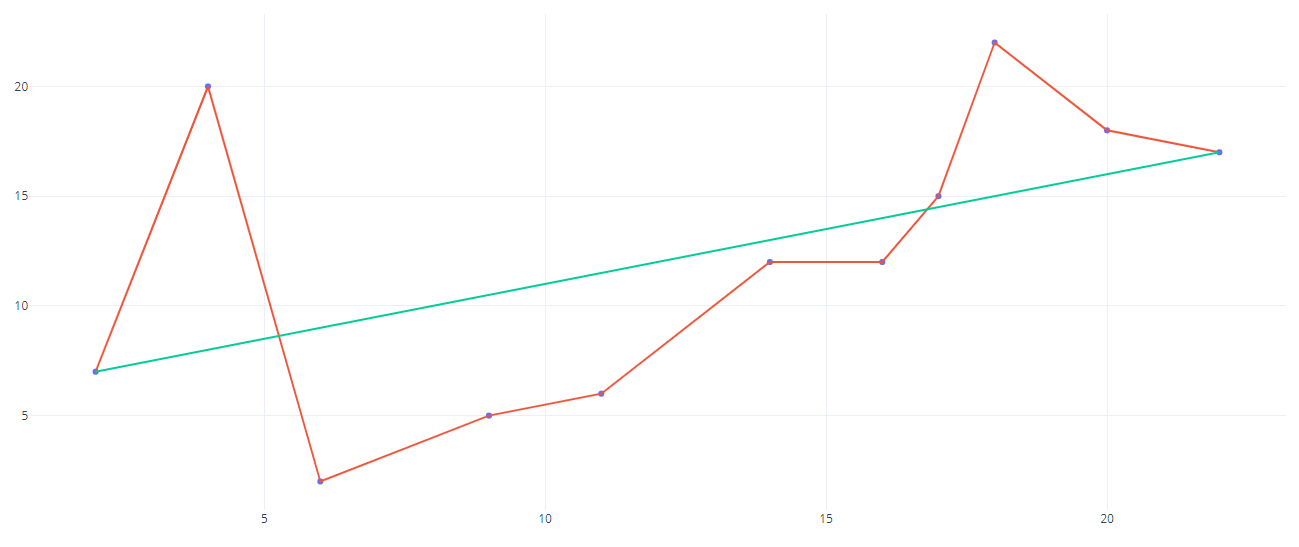
\includegraphics[width=\textwidth]{ermdiagram.png}
The figure above is a perfect example of overfitting as a result of Empirical Risk Minimisation. The green line shows the line of best fit of the predictive function which indicates how the function would best represent the data. The orange line is the same predictive function after attempting to minimise the empirical risk to it's lowest point. For the training data, the function will perform extremely well with almost no error however this is due to overfitting, resulting in the function to perform extremely poorly on the testing or real world data. For this particular case the Empirical Risk Minimisation would be giving a false representation of the true risk as it would appear to be a low empirical error when in reality it would be extremely high on unseen data. 


\section{Structural Risk Minimisation}
The principle of Structural Risk Minimisation (SRM) was introduced as an effective method of tackling the problem of overfitting in Empirical Risk Minimisation. This does so by making use of the VC-Dimension mentioned previously to analyse a prediction function's complexity and by using Empirical Risk Minimisation. The aim of this minimisation principle is to find the most optimal predictive function, which can be defined as the function with a low value of empirical risk and a low VC-Dimension (low complexity). This balance between these two bounds is the essence of Structural Risk Minimisation.

\section{Factors affecting Empirical Risk Minimisation}

From what can be seen there are several factors that indicate how good of an approximation of risk will be. Firstly, the size of the dataset. A small dataset will most likely lead to high bias and overfitting meaning a large dataset is preferred as it will provide a better approximation of the true distribution. The underlying distribution of the data will also affect the approximation as complex and irregular distributions will cause the function to overfit as previously mentioned. Another factor is the loss function used. The loss function should be consistent with the data and not show irregular spikes in loss values at certain data points. Lastly, another factor that affects empirical risk minimisation is the prediction function. If the function considered is large and complex, it will be a much more difficult task in finding the empirical risk and the true risk. 

\section{Conclusion}
In conclusion, the principle of Empirical Risk Minimisation is an effective way of minimising the empirical error of a prediction function. Under the appropriate conditions, by reducing this risk on a subset of the population data then the true risk will be reduced to the same extent. However, caution needs to be taken as to prevent the case of overfitting.

\bibliographystyle{plainnat}
\bibliography{empiricalriskminisation_nf}
\end{document}


